\documentclass[10pt]{article}
\usepackage[margin=1in]{geometry}
\usepackage{amsmath,amssymb}
\usepackage{booktabs}
\usepackage{siunitx}
\usepackage{graphicx}
\usepackage[colorlinks=true,linkcolor=black,citecolor=black,urlcolor=black]{hyperref}
\setlength{\parskip}{0.35em}
\setlength{\parindent}{0pt}

\begin{document}

\begin{center}
{\Large \textbf{Summer 2025 Research Summary}}\\[2pt]
{\large \textbf{Machine Learning Flags Fast Neutrino-Flavor Instabilities}}\\[4pt]
John McGuigan \quad Advisor: Sherwood Richers\\
Department of Physics and Astronomy, University of Tennessee, Knoxville\\

\textbf{Abstract.}
Core-collapse supernovae (CCSN) and neutron star mergers (NSM) host extreme conditions where neutrino self-interactions can trigger \emph{fast flavor instabilities} (FFI) on cm/ns scales.
I trained heavily regularized multi-layer perceptrons (MLPs; 4--6 layers, hundreds of neurons wide) in PyTorch on $\sim 8\times 10^5$ labeled snapshots spanning seeded-unstable, guaranteed-stable, and neutron-star-merger (NSM) cases.
After a systematic hyperparameter search (dropout, batch normalization, weight decay, batch size, learning rate schedules, and early stopping) and class-weighted training to address the $\sim$5--6\% unstable minority class, the best model reaches $F_1 \approx 0.95$ on held-out data while remaining small enough for in-situ use in simulation codes.
The network outputs a calibrated $P(\mathrm{FFI}\mid x)$ per grid cell, replacing an expensive dispersion solve with negligible overhead in principle; integration tests and wall-time benchmarks are planned for production hydrodynamics runs.

\subsection*{Background \& Physics}
Neutrinos carry away $\gtrsim 99\%$ of the gravitational binding energy in core collapse, and their angular electron-lepton-number (ELN) spectra can admit crossings that seed FFI.
In the mean-field limit, the flavor density matrix $\rho_{\mathbf{p}}$ is
\begin{equation*}
i\,\partial_t \rho_{\mathbf{p}} = \left[ H_{\mathrm{vac}} + H_{\mathrm{mat}} + H_{\nu\nu}, \, \rho_{\mathbf{p}} \right],
\end{equation*}
with the self-interaction term
\begin{equation*}
H_{\nu\nu} \propto \mu \!\int (1-\cos\theta)\, G(\mathbf{v})\, d\Omega,
\end{equation*}
where $G(\mathbf{v})$ is the ELN angular distribution and $\mu$ sets the interaction scale. The presence of ELN crossings can drive flavor conversion on microscopic (cm/ns) scales that are numerically difficult to resolve directly across all cells in neutrino transport simulations.

\subsection*{Data \& Features}
Labeled examples consist of $\sim 8\times 10^5$ per-cell snapshots (stable versus FFI-unstable) drawn from core-collapse supernovae (CCSN) and neutron star mergers (NSM).
The feature vector contains 27 scalars per cell: entropy; flux-integrated neutrino number and energy densities; all dot products among electron-neutrino and antineutrino flux moments up to second order; and ELN-crossing proxies. Density $\rho$ and electron fraction $Y_e$ are not included among the inputs.
The dataset is imbalanced with only $\approx$5--6\% unstable cells, and an 80/20 train/validation split with fixed folds and multiple deterministic seeds tests reproducibility.

\subsection*{Model \& Training}
The classifier is a fully connected multi-layer perceptron (MLP) with 4--6 hidden layers a few hundred neurons wide, using ReLU activations, BatchNorm, and dropout.
Training employs class-weighted binary cross-entropy loss with $L_2$ regularization,
\begin{equation*}
\mathcal{L} = -w_1\, y\log \hat y - w_0 (1-y)\log(1-\hat y) + \lambda \sum_{\ell}\lVert W_\ell\rVert_2^2,
\end{equation*}
and is optimized with AdamW and a cosine/step learning-rate schedule.
Batch sizes of $4\,096$--$16\,384$ start near $3\times 10^{-3}$ learning rate with decay and early stopping to prevent overfitting.
After training, the classification cutoff on $P(\mathrm{FFI}\mid x)$ is swept to maximize the $F_1$ score, balancing precision and recall.

\begin{figure}[h]
    \centering
    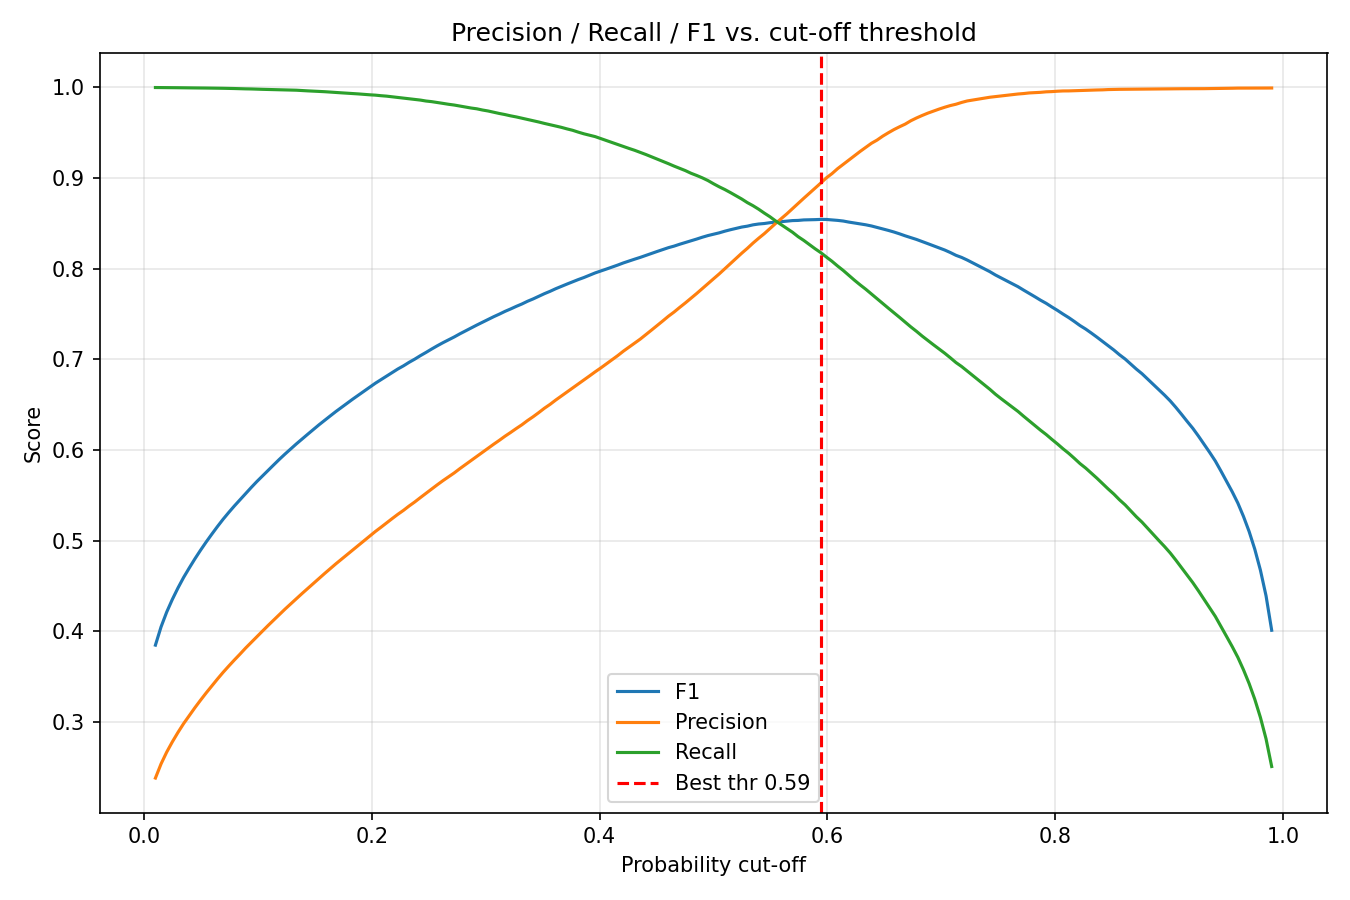
\includegraphics[width=0.6\textwidth]{cutoff_sweep.png}
    \caption{Validation $F_1$ score versus classification cutoff.}
\end{figure}

\subsection*{Validation \& Reproducibility}
Precision, recall, and $F_1 = \frac{2PR}{P+R}$ are measured on a held-out test set.
Results at the optimal cutoff remain stable across seeds; representative numbers are below.

\begin{center}
\begin{tabular}{@{}lccc@{}}
\toprule
Seed & Recall & Precision & $F_1$ \\\midrule
17 & 0.921 & 0.983 & 0.951 \\
43 & 0.919 & 0.974 & 0.945 \\
\bottomrule
\end{tabular}
\end{center}

Median performance across top configurations sits near $F_1 \approx 0.94$--$0.95$ with high precision ($\approx$0.97--0.98) and strong recall ($\approx$0.90--0.92).
I also trained smaller variants (fewer layers and narrower widths) to minimize inference cost; these retain competitive $F_1$ with modest drops in recall.

\subsection*{Deployment Plan \& Impact}
For in-situ prediction, the model is exported to TorchScript and run as batch per-cell inference on CPU or GPU within radiation-hydrodynamics codes.
The resulting $P(\mathrm{FFI}\mid x)$ serves as a flag or risk score that enables flavor-aware closures or triggers higher-fidelity solvers only where instability is likely.
The architecture is constrained for real-time deployability, and end-to-end wall-time benchmarks on production grids are the next step.

\subsection*{Progress to Date}
I built an end-to-end PyTorch training pipeline with data loaders, augmentation hooks, logging, and plotting.
Automated hyperparameter searches span depth, width, dropout, weight decay, batch size, and learning-rate schedules with early stopping.
Class-weighted training handles severe imbalance, and threshold sweeps with calibration curves set operating points.
Reproducibility studies across multiple seeds provide convergence diagnostics and overfitting detection.
I also developed compact models that retain high sensitivity to the minority class while enabling faster inference.

\textbf{Next Steps.}
Runtime profiling inside a test hydrodynamics code; uncertainty calibration (temperature scaling, isotonic regression), out-of-distribution checks for new progenitors/NSM conditions, and active-learning loops that prioritize follow-up dispersion solves where the classifier is uncertain.
\end{center}

\end{document}
